\documentclass[a4paper, oneside, 12pt, titlepage]{article}

\usepackage[utf8]{inputenc}
\usepackage[T1]{fontenc}
\usepackage{amsmath}
\usepackage{array}
\usepackage{amsfonts}
\usepackage{tikz}
\usepackage[inline]{enumitem}
\usepackage{varwidth}

\usetikzlibrary{arrows}

\begin{document}

\title{Formalizing \emph{Types and Programming Languages} in Isabelle/HOL}
\author{Martin Desharnais}
\maketitle

\begin{abstract}
We formalized, using Isabelle/HOL, some languages presented in the first two sections, namely
"Untyped Systems" and "Simple Types", of the book \emph{Types and Programming Languages} by
Benjamen~C.~Pierce. We first begin with a short tour of lambda-calculus, type theory and the
Isabelle/HOL theorem prover before attacking the formalization per se. Starting with an arithmetic
expression language offering booleans and natural numbers, we pursue, after a brief digression to
the "de Bruijn indices", to the untyped lambda-calculus. We then return to a typed variant of the
arithmetic expression language before to conclude with the simply typed lambda-calculus.
\end{abstract}

\tableofcontents
\newpage

\section{Introduction}

This bachelor thesis deals with the formalisation, in the Isabelle/HOL theorem prover, of part of
the book \emph{Types and Programming Languages}, hereafter abbreviated \emph{TAPL}, by
Benjamen~C.~Pierce. This work concentrate on four of the languages, ranging from simple arithmetic
expressions to fully fledged lambda-calculus, presented in the first two sections, namely "Untyped
Systems" and "Simple Types".

The main motivation to have chosen this subject is the intersection of personal interested and of
opportunities provided by our intership at the chair for logic and verification at TU München.
Having gradually developped an interest for programming languages in the last years, we were eager
to learn more about the foundations of type theory. Pierce's book stand out as a reference
recommended for a deep introduction to the main elements of the field. Also, as part of our
intership, we worked on the implementation of the (Co)datatype module in the Isabelle/HOL theorem
proover. Having experienced the implementator role, we also wanted to learn about the user role and
about the process of formalization. The choise of this subject for this thesis was thus a logic
consequence.

Before to dig into the realm of formalizations, we first introduce the required background (section
\ref{sec:background}) in lambda-calculus, type systems and Isabelle/HOL. The lambda-calculus is a
core calculus that captures the essentials features of programming languages. That is, there exists
a way to encode high level features such as recursion, datatypes, references, etc. Such calculus can
come, as prorgramming languages, in two variant: typed and untyped. A type system is a syntactic
method to prove the absence of certain behaviors such as the misusage of objects of a certain nature
(e.g. natural numbers, booleans, string of characters, etc.) To formalize those we used
Isabelle/HOL, an interactive theorem prover based on higher order logic. It resembles a programming
language in that one can define datatypes and functions. The difference is that it allows to
postulate properties of the formelly defined elements and to provide machine checked poofs that
those properties are theorems.

The formalizations we performed all have a direct corespondance with chapters from \emph{TAPL}
(section \ref{sec:structure-of-formalization}). We provide one Isabelle/HOL theory file per chapter
and introducte them in the same order. The only exception is the nameless representation of terms
that we introduce earlier because our formalization depent on it while, in the book, it is an
independant subject.

The untyped arithmetic expressions language (section \ref{sec:untyped-arith-expr}) served as a
warm-up to experiment with the general structure of formalizations. It consists of boolean
expressions and natural numbers. This simplicity allows to concentrate on the the important
definitions and to accustoms ourself with the notation. Most of our definitions and theorems closely
follows the ones from the book. The main exceptions being that we explicitly expause some hypothesis
that are implicit in the book and our slightly different definition for the mutli-step evaluation
relation.

The formalization (section \ref{sec:nameless-rep-of-terms}) of the nameless representation of terms,
also known as "de Bruijn indices", was not initially planned but arose from the need to use a
concreate representation for variables in the lambda-calculus. Our formalization closely follows the
book.

While the previous formalizations were either a warm-up or a representation necessity, the untyped
lambda-calculus (section \ref{sec:untyped-lambda-calculus}) is the first core calculus we
formalized. This formalization is the first where we differ from the book in a non-negligible way.
As presented, the evaluation relation assumes that names clashes in variables are automatically
solved by renaming them and, thus, ignore this possibility from there on. Such an assumption is not
accepted for a computer-verified proof. We choosed to use "de Bruijn indices" as representation for
variable to encode this assumption. Also, since the chapter is more focused on explaining the lambda
calculus, it does not contain theorems as the other chapters. Nevertheless, we decide to reprove, or
disprove, the theorems introduce with the arithmetic expressions language.

The typed arithmetic expressions language (section \ref{sec:typed-arith-expr}) is again a warm-up;
this time, to experiment with the formalization of a type system. Our formalization closely follows
the book.

The simply typed lambda-calculus (section \ref{sec:simply-typed-lambda-calculus}) is the second core
calculus that we formalize. Here, we differ significantly from the book. Mainly because of our use
of "de Bruijn indices" but also because of our reprensentation of the typing context, we needed to
adapted some lemmas and replace others. This was quite challenging since we then could not follow
the described proofs anymore and had to find the right assumptions for our lemmas. We belive that
our formalization still respect the spirit of the book since only the helper lemmas changed and the
theorems remains the same.

\section{Background}
\label{sec:background}

\subsection{Lambda-Calculus}

The lambda-calculus is a minimalist language, where everything is a functions, that can be use as a
core calculus capturing the essential features of complex programming languages. It was formulated
by Alonzo Church \cite{???} in the 1930s as a model of computability. At the same time, Alan Turing
was formulating what is now known as a Turing machine \cite{???} for the same purpose. It was later
proved that both systems are equivalent in expressive power \cite{???}.

As a programming language, it can be intriguing at first because everything reduces to function
abstraction and application. The syntax comprises just three sorts of terms: variables, function
abstractions over a variable and applications of a term to an other. Those three constructs are
summarized in the following grammar using a BNF-like notation.

\begin{align*}
  \lambda\text{-term} ::= & \\
    & x && \text{variable} \\
    & \lambda x. t && \text{abstraction} \\
    & t_1 \text{ } t_2 && \text{application}
\end{align*}

Following are a few standard $\lambda$-term show as examples of how the grammar is actually used.

\begin{align*}
  & \lambda x. x && \text{identity} \\
  & \lambda x. \lambda y. x && \text{constant} \\
  & \lambda x. \lambda y. x \text{ } y \text{ } y && \text{double application} \\
  & \lambda x. \lambda y. \lambda z. x (y \text{ } z) && \text{function composition}
\end{align*}

Having no built-in constant or primitive operators (e.g. numbers, arithmetic operations,
conditionals, loops, etc.), the only way to "compute" something is by function application (also
known as $\beta$-reduction and noted $\to_\beta$). It consists of replacing every instance of the
abstracted variable in the abstraction body by the effective argument. Following is an example of a
$\lambda$-term that can be reduced twice.

\begin{align*}
  (\lambda x. (\lambda y. y) x) ((\lambda w. w) z)
    & \to_\beta (\lambda x. (\lambda y. y) x) z \\
    & \to_\beta (\lambda y. y) z \\
    & \to_\beta z
\end{align*}

This apparently simple operation hide a complex corner case: name clashes. Nothing prevent two
functions from using the same name for there abstracted variable. One can not simply replace every
variable with the same name when performing a substitution but must also take variable scopes into
account. Here is a simple example that demonstrate that a naïve approche can fail to preserve the
semantic of the original $\lambda$-term.

\begin{displaymath}
  (\lambda x. \lambda y. x) y \not\to_\beta \lambda y. y \\
\end{displaymath}

One solution to this problem is to rename function arguments when necessary (also known as
$\alpha$-equivalence and noted $=_\alpha$). Here is a correct $\beta$-reduction for the previous
example.

\begin{align*}
  (\lambda x. \lambda y. x) y
    & =_\alpha (\lambda x. \lambda w. x) y \\
    & \to_\beta \lambda w. y \\
\end{align*}

The difference is important. Under the naïve approche, the $\lambda$-term was wrongly reduced to the
identity function while the correct reduction lead to a function return the constant $y$.

Many constructions from high level programming languages can be encoded using only those basic
features.  Unary functions are already supported and n-ary functions can be straitforwardly emulate
by having a function return an other function as was done in the previous examples.

\begin{displaymath}
  \text{n-ary function} \equiv \lambda x_1. \lambda x_2 \dots \lambda x_n. t
\end{displaymath}

An other common construction is a \emph{let binding} which serves to attach an identifier to a
complex expression. It can be emulated in lambda-calculus with a single function abstraction.

\begin{displaymath}
  \text{let } x = y \text{ in } t \equiv (\lambda x. t) y
\end{displaymath}

Although significantly less obvious, it is also possible to express booleans only with functions.
The encoding is based on the idea that any use of booleans can be express with only three
primitives: a constant representing a true value, a constant representing false values and an
operation to choose between two alternatives.

\begin{align*}
  \text{true}
    & \equiv \lambda t. \lambda f. t \\
  \text{false}
    & \equiv \lambda t. \lambda f. f \\
  \text{if } b \text{ then } t \text{ else } e
    & \equiv \lambda b. \lambda t. \lambda f. b \text{ } t \text{ } f
\end{align*}

Using the rules already discussed, it is trivial to show that the following reduction is valid.

\begin{displaymath}
  \text{if true then } x \text{ else } y \to_\beta \dots \to_\beta x
\end{displaymath}

Other encodings exists for constructions such as numbers, list, datatypes, arbitrary recursion, etc.

\subsection{Type Systems}

Type systems are a syntactic method to prove the absence of certain behaviors. They differ from
testing in that they are exhaustive and automatic. In this context, exhaustiveness means that each
checked invarient is proved to hold for the complete program instead of focusing on a single unit of
code. Automaticness means that the process is non-interactive, i.e. the algorithm does not need
other informations than what it can find in the source code of the program.

The kind of errors detected depend on the specific type system under consideration, but can range
from fairly simple to very complex. Examples of simple errors include typographical mistakes, usage
of values of the wrong kind (see figure \ref{fig:simple-type-mismatch} for an example) and usage of
undefined operations. With Sufficiently powerfull type systems, specific requirements can be provide
as type annotations. Example of such include that the output list of a sorting function be a
permutation of the input list, that the argument of an indexing operation on a list be in a valid
range or that two multiplied matrixes have compatible dimenssions. The more information one put in
the types, the more invalid programs the type checker will catch, but the more work will be required
by the programmer to convince the algorithm that the program fullfill it's specifications. An
important design decision when defining a type system is to find a tradeoff between those two
conflicting properties.

\begin{figure}[h]
  \begin{center}
    \begin{tabular}{m{3.5cm} | m{5.5cm}}
      $\text{add} : \mathbb{N} \to \mathbb{N} \to \mathbb{N}$ \newline
      $\text{true} : \mathbb{B}$ \newline
      add true true
      & error in function application, "add" expects a $\mathbb{N}$ but a $\mathbb{B}$ was provided
    \end{tabular}
  \end{center}
  \caption{Simple type mismatch in function application}
  \label{fig:simple-type-mismatch}
\end{figure}

Since they are often bundle with the compiler of a programming language and, thus, part of the
normal programming cycle, they allow early detection of programming errors. Moreover, the diagnoses
of type checkers can often pointed accuratly the source of the error, at the difference of run-time
tests where the effect of an error can sometime be visible only much farther in the code when
something start to go wrong.

An other important way in which type systems can be use is as an abstraction tool. It is widely
accepted that, in the context of large scale software developpement, the program should be split
into distinct modules that communicate through an interface. Types are an natural fit to serve as
such an interface. Enven in smaller scale programming, it is usefull to caracterise a datatype not
by the way it is implemented but by the different operations that can be perform on it, also known
as abstract datatypes).

Types can also be use an invaluable maintenance tool. More informally, they serve as a checked
documentation of programs and, being simpler thant the computation they caracterise, they can help
to reason about such computation on a higher level. But they can also serve a very practical
purpose, by checking which part of a program is affected by a change. If one decides to change the
arguments of a function or remove a field in a structure, a simple type checking pass will provide
an exhaustive list of the places that need to be updated to cope with the modification.

% Language safety is a very desirable property of programming language that can be achived by type
% systems.
%   * e.g. memory safe
%   * A safe language is completly defined by its programmer manual.
%     * C contains a lot of implementation defined and undefined behaviours.

Due to their static nature, type systems are conservatives in that they will always reject bad
programs at the expence of something rejecting good programs. A simple example of such limitation is
the the following program will fail to typecheck, even if it happens that that the complex boolean
expression will always evaluate to true at runtime.

\begin{displaymath}
  \texttt{if} <\text{complex-expression}> \texttt{then } 42 \texttt{ else } \text{true}
\end{displaymath}

Having only access to static information, a type checker only see that a boolean can take two
different values and, thus, must insure that the program is valide in both cases. In this example,
this implies that both branch of the \texttt{if} must be well-typed and that their type must be the
same. It is the main goal of type theory scientists to develop type systems in which more more valid
programs are accepted while more invalid programs are rejected.

\subsection{Isabelle/HOL}

The theorem proving community can be subdivise in two groups: automatic theorem proving (ATP) and
interactive theorem proving (ITP). Each have their own set of motivation, goals, methodologies and
tools. In ATP, one must formulate it's context and equations in some logical formalisms and ask the
theorem to find a proof. The limiting factor will be the algorithm used by the tool. Example of such
provers include Z3, Vampire and SPASS. In ITP, one must also formulate it's context and equations in
some logical formalisms, although usually a stronger one, and will give instructions guiding the
prover, which explain the usual name of proof assistant. Here, the limiting factor will be the
ability of the human to guide it's tool. Example of interactive theorem provers include Isabelle,
Coq and Agda provers and the proof assistants.

Isabelle is a generic interactive theorem prover for implementing logical formalisms and
Isabelle/HOL is its specialization to higher order logic. We will now present the main notions
needed to read the comming formalizations. To this end, we will establish a comparaison with typical
programming languages from the ML family.

A Isabelle theory file serve as the basic unit of encapsulation of formalizations and reusable
libraries. Is analogous to modules in programming languages. Every definition and theorems
developped must belong to a theory and can be made accessible to other theories by importing them.

Types and function definitions serve to describe entities and how to operate on them. They work in
very similar way to their counterpart in functional programming languages. A new type is introduce
with the \texttt{datatype} command, followed by the name of the type and the different constructors
separated by a \texttt{|}. Following is the standard definition of the parametric \texttt{list}
datatype.

\begin{verbatim}
datatype 'a list = Nil | Cons 'a "'a list"
\end{verbatim}

Definitions can take many forms in isabelle/HOL. A primitively recursive function is introduced with
the \texttt{primrec} command and defined by pattern matching over its arguments. Each pattern match
entry must then provide the value to which the function evaluate. Following is a definition of the
\texttt{ordered} higher order function which checked if all the elements of a lis are ordered with
respect to a binary predicate provided as an argument.

\begin{verbatim}
primrec ordered :: "('a => 'a => bool) => 'a list => bool" where
  "ordered f Nil = True" |
  "ordered f (Cons x xs) = (case xs of
     Nil => True |
     Cons y ys => f x y /\ ordered f xs)"
\end{verbatim}

An way in which this function could have been defined is with an inductive definition. Introduced
with the \texttt{inductive} command, it allows to express boolean functions by providing an
inductive definition of when the function should evaluate to true, leaving all the other cases to
false. The definition consists of a base case and possibly many inductive cases. Following is the
same function, named \texttt{ordered'} this time, using an inductive definition.

\begin{verbatim}
inductive ordered' :: "('a => 'a => bool) => 'a list => bool" where
  "ordered' f Nil" |
  "ordered' f (Cons x Nil)" |
  "f x1 x2 ==> ordered' f (Cons x2 xs) ==> ordered' f (Cons x1 (Cons x2 xs))"
\end{verbatim}

Theorems, also named lemmas, are true facts involving the defined elements. They could be compare to
the asserts used in programming languages. The main difference is that asserts are validate by
evaluating the expression while theorems are validate by a formal proof. This is the point where the
analogy with programming languages stops since this concept is unique to theorem provers. In
Isabelle/HOL, a proof can take two forms: a low-level sequence of \texttt{apply} steps or
higher-level structured definition. Following is an example of a lemma that proved, using the
low-level style, that the list of increasing natural numbers are ordered with respect to the usual
comparison operation.

\begin{verbatim}
lemma "ordered (%x y. x < y) (Cons (1 :: nat) (Cons 2 (Cons 3 (Cons 4 Nil))))"
  apply (unfold ordered.simps)
  apply (unfold list.case)
  apply (rule conjI, simp)+
  apply (rule TrueI)
done
\end{verbatim}

This proof is easilly verified by a computer but very hard to read for a human. For this reason,
the Isabelle/Isar structured proof language was designed to allow the writing of more human-friendly
proofs. Following is a theorem that, whenever the \texttt{ordered} function returns true for a given
predicate and list, the \texttt{ordered'} function will also return true.

\begin{verbatim}
theorem primrec_imp_inductive:
  "ordered f xs ==> ordered' f xs"
proof (induction xs rule: list.induct)
  case Nil
  thus ?case by (auto intro: ordered'.intros)
next
  case (Cons x xs)
  thus ?case by (cases xs rule: list.exhaust) (auto intro: ordered'.intros)
qed
\end{verbatim}

This proof is still easilly verified by a computer but it is also more readable for a human. It is
easy to see that the proof work by induction on the list \texttt{xs}, that the base case is first
proved and that the inductive case required to consider the exhaustive list of value the argument
\texttt{xs} can take.

This section only presented the most used constructions in the formalizations described in this
thesis. For a real introduction to Isabelle/HOL, the reader is encourage to start with the tutorial
\cite{???} distributed with the system and continue, for a deeper understanding, with the more
exaustive manual \cite{???}.

\section{Structure of the Formalization}
\label{sec:structure-of-formalization}

We formalized six chapters of the first two sections of TAPL. Figure \ref{fig:TAPL-toc} presents the
table of content of those two sections --- the formalized chapters are in bold --- and figure
\ref{fig:TAPL-dependencies} present the dependencies between the chapters; a normal arrow imply a
direct dependency while a dashed arrow only imply that the knowledge learned in one chapter is
usefull for an other.

\begin{figure}[h]
  \footnotesize
  \centering
  \begin{varwidth}{\textwidth}
    \begin{enumerate}[label=\Roman*]
      \itemsep 1pt
      \item Untyped Systems \hfill
        \begin{enumerate}[label=§ \arabic*]
          \setcounter{enumii}{2}
          \item \textbf{Untyped Arithmetic Expressions}
          \item An ML Implementation of Arithmetic Expressions
          \item \textbf{The Untyped Lambda-Calculus}
          \item \textbf{Nameless Representation of Terms}
          \item An ML Implementation of the Lambda-Calculus
        \end{enumerate}
      \item Simple Types \hfill
        \begin{enumerate}[label=§ \arabic*]
          \setcounter{enumii}{7}
          \item \textbf{Typed Arithmetic Expressions}
          \item \textbf{Simply Typed Lambda-Calculus}
          \item An ML implementation of Simple Types
          \item Simple Extensions
          \item Normalization
          \item References
          \item Exceptions
        \end{enumerate}
    \end{enumerate}
  \end{varwidth}
  \caption{Section I and II of TAPL}
  \label{fig:TAPL-toc}
\end{figure}

\begin{figure}[h]
  \begin{center}
    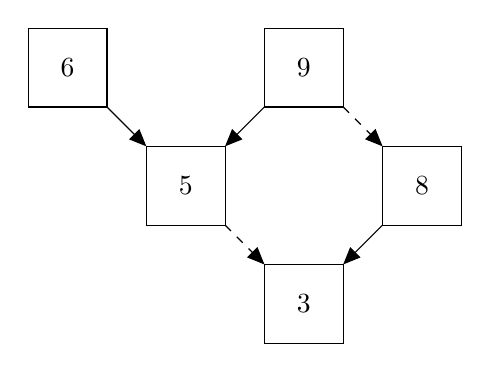
\begin{tikzpicture}[>=triangle 45]
      \draw (0,3) rectangle (1,4) node[pos=0.5]{6};
      \draw (1.5,1.5) rectangle (2.5,2.5) node[pos=0.5]{5};
      \draw (3,0) rectangle (4,1) node[pos=0.5]{3};
      \draw (3,3) rectangle (4,4) node[pos=0.5]{9};
      \draw (4.5,1.5) rectangle (5.5,2.5) node[pos=0.5]{8};
      \draw [->] (1,3) -- (1.5,2.5); % 6 -> 5
      \draw [->, dashed] (2.5,1.5) -- (3,1); % 5 -> 3
      \draw [->] (3,3) -- (2.5,2.5); % 9 -> 5
      \draw [->, dashed] (4,3) -- (4.5,2.5); % 9 -> 8
      \draw [->] (4.5,1.5) -- (4,1); % 8 -> 3
    \end{tikzpicture}
  \end{center}
  \caption{Dependencies between the chapters of TAPL}
  \label{fig:TAPL-dependencies}
\end{figure}

The formalization closely follows the structure of the book. We provide one Isabelle theory file per
chapter and mainly introduce them in the same order. The only exception is the chapter on "Nameless
Representation of Terms". In the book, it is treated as completely separate issue from the chapters
on lambda-calculus. They present it as a concrete alternative to the implicit $\alpha$-conversion
they assumes in there proofs. Since we chose this representation for our formalization, we had to
diverge from the book and introduce this subject prior to the untyped lambda-calculus. Figure
\ref{fig:thys-dependencies} presents the dependencies between our Isabelle theory files.

\begin{figure}[h]
  \begin{center}
    \begin{tikzpicture}[>=triangle 45]
      \draw (0,3) rectangle (1,4) node[pos=0.5]{6};
      \draw (1.5,1.5) rectangle (2.5,2.5) node[pos=0.5]{5};
      \draw (3,0) rectangle (4,1) node[pos=0.5]{3};
      \draw (3,3) rectangle (4,4) node[pos=0.5]{9};
      \draw (4.5,1.5) rectangle (5.5,2.5) node[pos=0.5]{8};
      \draw [->, dotted] (1.5,2.5) -- (1,3); % 5 -> 6
      \draw [->, dashed] (2.5,1.5) -- (3,1); % 5 -> 3
      \draw [->] (3,3) -- (2.5,2.5); % 9 -> 5
      \draw [->, dashed] (4,3) -- (4.5,2.5); % 9 -> 8
      \draw [->, dotted] (4.5,1.5) -- (4,1); % 8 -> 3
    \end{tikzpicture}
  \end{center}
  \caption{Dependencies between the theory files}
  \label{fig:thys-dependencies}
\end{figure}

It was possible to directly base the typed arithmetic expressions on untyped arithmetic expression
by importing the theory and reusing its definition. This is represented as a dotted arrow in figure
\ref{fig:thys-dependencies}. This reuse was possible because, for this language, types are external
to the representation of terms. For the typed lambda-calculus, on the contrary, we needed to alter
the representation of terms to add the typing annotation on abstraction variables, thus preventing
the reuse of the untyped lambda-calculus theory.

\section{Untyped Arithmetic Expressions}
\label{sec:untyped-arith-expr}

  * Most our definitions closely follow the ones presented in the book
    * With the exception that some information implicit in the book must be explicitly state.
      * e.g. "nv" that stand for numeric value must be a "is\_numeric\_value nv" assumption.
    * The multistep evaluation relation is defined differently, take the shape of a list.
      * With a base reflexive case (Nil)
      * And a progress case (Cons)
      * We then supply lemmas showing that our definition exibit the same properties as the one in
        the book.

  * We had to introduce an helper lemma (eval\_once\_size\_B) that was implicit in the book about the
    fact that each evaluation step reduce the size of the term.

  * The formalization is separate in two, with first only booleans and then the fully fledged
    arithmetic expression language.
    * The second part is just an explanation and does not contains any theorems.
      * We decided to reprove, or disprove, the theorems introduced in the section on booleans.
  * Lemma 3.3.3: We choose to make an induction on the structure of terms instead of the depth.

  * Lemma 3.3.4: Trivial because already provided by Isabelle/HOL modulo schematic variable
    instanciation.

\section{Nameless Representation of Terms}
\label{sec:nameless-rep-of-terms}

  * Representation of variable which free us to consider the case of variable name clashes.

  * Abs "x" (Var "x") = Abs (Var 0)
  * Abs "x" (Abs "y" (Var "x")) = Abs (Abs (Var 1))

  * We defined a single shift function for both up and down shift.
    * It use a integer as a shift size and we convert it to a natural number when need.
      * rely on the fact that "nat (int 2 - 5) = 0" instead of -3
    * It caused small difficulties in Typed Lambda-Calculus because we had to handle both case in
      our proofs even if we were interested in only one.

\section{Untyped Lambda-Calculus}
\label{sec:untyped-lambda-calculus}

  * The main point of this chapter is the presentation of the lambda-calculus and explanations of
    why it is so important as a basic representation of programming languages.

  * The fact that Church numerals, booleans, etc. represent the real numerals and booleans took me a
    while to understand.
    * The main point of the story is that, we tend describe a concept through what can be achived
      with it i.e. the operations that are available
    * Church encoding is isomorphic to their natural counterpart because we can make the exact
      operations and change freely from one representation to the other.

  * Def 5.3.1 is quite different because we chose De Bruijn indices.
    * FV : term -> var set

  * The substitution is very different because we use De Bruijn indices while the book assumes
    alpha-conversion when necessary.
    * It did not caused problems in this chapter (but wait for simply typed lambda-calculus...)

  * I was quited shocked when I realised that the given definition of the small-step evaluation
    relation does not allow the beta reduction of (%x. x) y to y.
    * I later realized that it is explained by the concept of bounded variables, free variables and
      closed terms.

  * The chapter does not contain theorems on the language per se, so we decieded to reprove, or
    disprove, the theorems introduced in the section on booleans.

\section{Typed Arithmetic Expressions}
\label{sec:typed-arith-expr}

  * The formalisation of this chapter trivially follow the book.

\section{Simply Typed Lambda-Calculus}
\label{sec:simply-typed-lambda-calculus}

  * We chose to represent the typing context as a (type list).
    * which is equivalent to ((nat * type) * set)
    * while the book use ((string * type) * set)

  * I was shocked when I realized that the pure simply typed lambda-calculus is degenerated.
    * i.e. It have to be extand with some basic datatype to be used.
    * Booleans in our case

  * Thm 9.3.5[Progress] This is the first place where we explicitly had to state that the term is
    closed

  * Lemma 9.3.6[Permutation of context] is not a theorem in our chose representation of typing
    context.
    * Fortunatly, we manage without it.

  * Lemma 9.3.7[Weakening of context] the form is quite different because of De Bruijn indices.
    * Was difficult to come with.

  * Lemma 9.3.7[preservation under substitution] the theorem (not just the form) is different.

  * We needed to add an other helper lemma, shift\_down, to prove thm 9.3.9
    * Was horrible to come with and even more horrible to prove

  * We also needed to add FV\_shift and FV\_subst helper lemmas
    * Was moderatly difficult to come with and prove

  * Thm 9.3.9[Preservation] Was very difficult to prove because, we did not had the required helper
    lemmas (see above).
    * Once the helper lemma were provided, the proof went quite smoothly.

  * For the part on type erasure, we had to define a new untyped lambda calculus because of the
    booleans.
    * While the book only provide definitions and proofs for a subset of the simply typed lambda
      calculus, our machined checked proofs required exhaustiveness.

\section{Conclusion}

\end{document}
